\section{Background}
\label{sec:background}

\subsection{Counterpoint}

\begin{figure*}
  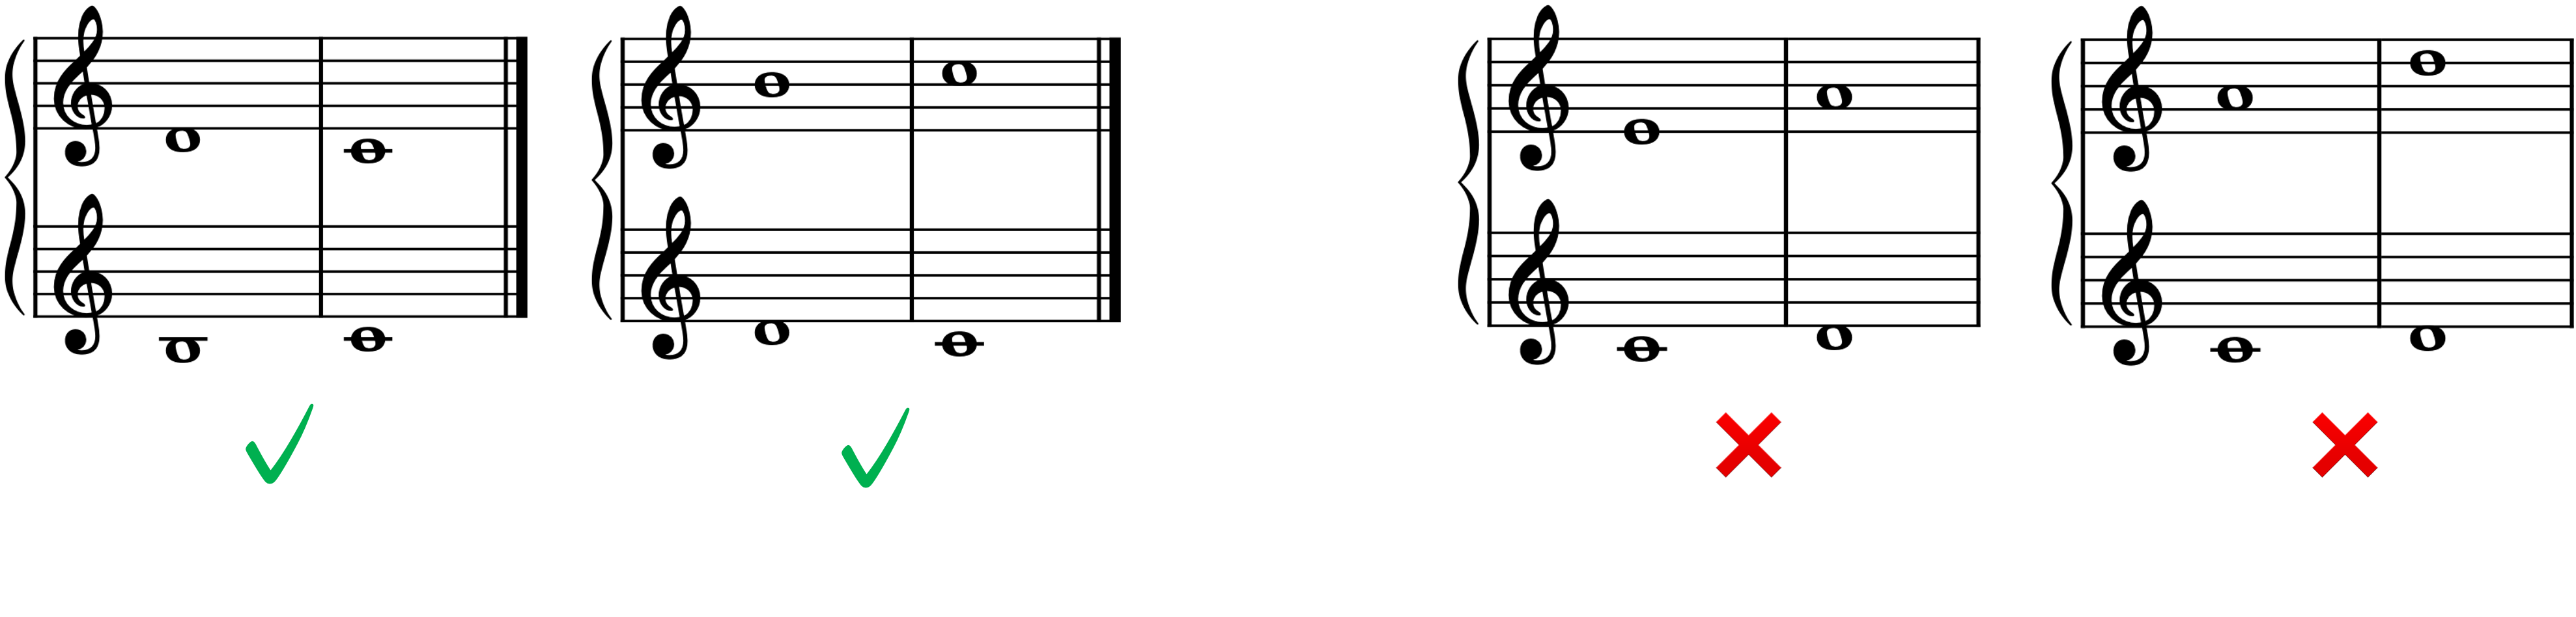
\includegraphics[width=16cm]{rules.png}
  \vspace{-6mm}
  \caption{Key Rules of First-Species Counterpoint}
  \label{fig:rules}
\end{figure*}

Counterpoint is an approach to composing music with multiple voices.
Species counterpoint is a method for learning how to compose
counterpoint, and first-species counterpoint is the simplest variant
consisting of two melodies sharing the same rhythm.
Composing counterpoint goes by picking a pre-existing melody called
\emph{cantus firmus} and writing a counterpoint line either above or
below the cantus firmus.
Here is an example of first-species counterpoint composed against a
phrase from the German song \emph{Froschgesang}.

\smallskip

\begin{center}
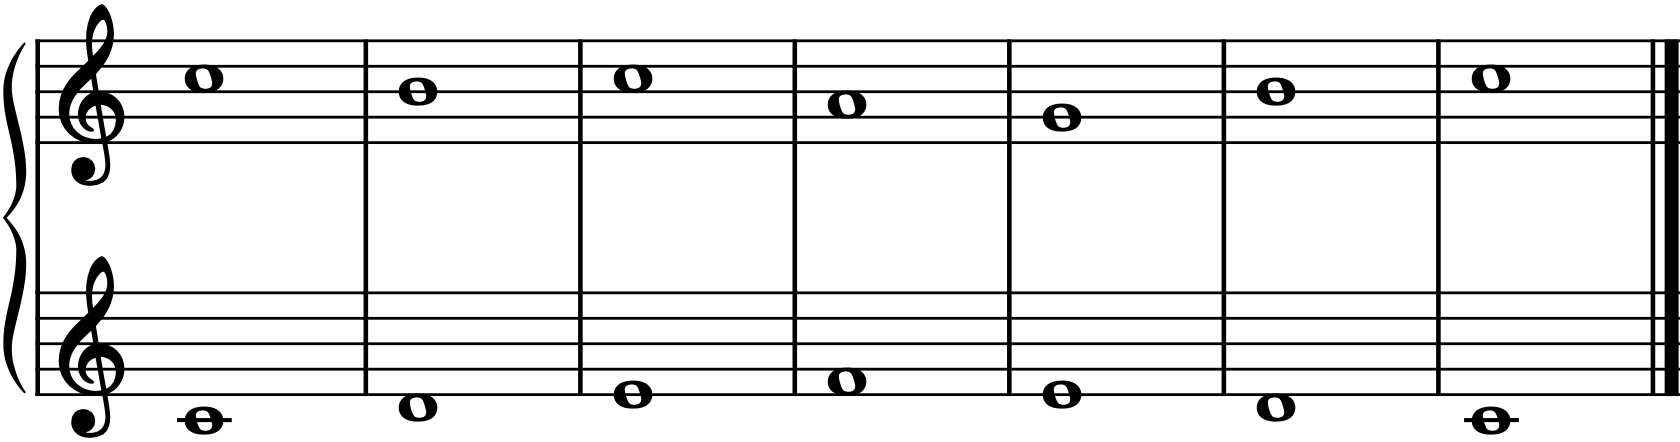
\includegraphics[width=7cm]{cp.png}
\end{center}

\smallskip

To compose good sounding counterpoint, one must follow certain rules.
Below are two key rules of first-species counterpoint given by
Fux~\cite{fux-cp}.

\begin{itemize}
  \item \textbf{End with a cadence.}
    The last interval must be either a unison or an octave, and it
    must be approached by stepwise contrary motion
    (Figure~\ref{fig:rules} left).
    The required progression is called a cadence, and it creates a
    sense of resolution.
    
  \item \textbf{No direct fifth or octave.}
    Fifths and octaves cannot be approached when the two voices move
    in the same direction (Figure~\ref{fig:rules} middle).
    The forbidden progression is called a direct fifth or octave, and
    it destroys the independence of the voices.

  \item \textbf{No successive large leaps in the same direction.}
    The counterpoint line should not move in a certain direction by
    successive large intervals, namely fifths and sixth
    (Figure~\ref{fig:rules} right).
    Such a motion disrupts the flow of the melody.
\end{itemize}

\subsection{Finite-Choice Logic Programming in Dusa}

Finite-choice logic programming~\cite{martens2025finite} is a new
foundation for writing logic programs that combine deductive specification 
and mutual-exclusion constraints. The meaning of such a program, rather
than a single canonical model, is the full {\em collection} of models
consistent with the theory represented by the program. This paradigm is
similar to that of answer set programming~\cite{lifschitz2019answer},
but it more naturally supports the characterization of
{\em infinite} collections of satisfying models, and a corresponding
operational model that stochastically explores the search space of
these models, producing them lazily. This operational model is realized by
the Dusa implementation. % TODO add web link

A Dusa program, like all logic programs, consists of a collection
of logical {\em rules} and {\em facts} that specify valid deductions
over a custom domain of {\em predicates}. Predicates in Dusa
may be associated with unique {\em values} (in which case we
sometimes refer to them as {\em attributes}). For example, in 
the domain of counterpoint, we use the predicate
\verb|cp T is I| to mean ``the counterpoint voice
at time step \verb|T| has interval \verb|I|.'' 
The \verb|is| keyword represents a uniqueness constraint, i.e. that for any
time point \verb|T|, there can only be one \verb|I| such that \verb|cp T is I|.

A {\em rule} is a schema for deduction that may use {\em logic variables}
(written beginning with capital letters, by convention) that are implicitly
universally quantified over the scope of the whole rule. Here is an
example (not an actual rule in our system):

\begin{verbatim}
cp T is I :- cf T is N, plus N 2 is I.
\end{verbatim}

One can read the \verb|:-| symbol as a ``backwards implication''
and the comma \verb|,| as conjunction. Thus,
this rule says that whenever the cantus firmus at time step \verb|T| is the
note \verb|N|, and the sum of \verb|N| and $2$ is \verb|I|, 
it {\em must} be the case that the counterpoint at time step
\verb|T| is \verb|I|. The comma-separated predicates to the right of the
\verb|:-| symbol are the {\em premises} of the rule, and the
single predicate to its left is the {\em head} of the rule.

A {\em fact} is simply a rule with no premises. In Dusa,
every logic variable appearing in the head of a rule must
occur in its premises, so facts must mention only {\em ground terms}, those
that do not contain any logic variables. For example, here is a fact
that asserts the counterpoint interval at time step $0$ is
a fifth:

\begin{verbatim}
cp 0 is fifth.
\end{verbatim}

\subsubsection{Choice Rules}

The main distinguishing feature of finite-choice logic
programming is the use of {\em choices} in rules, which
describe a set of mutually-exclusive assignments from
attributes to values. For example, the following rule
defines a predicate \verb|my_interval| which can take on
and of \verb|third|, \verb|fifth|, or \verb|unison|
as values:

\begin{verbatim}
my_interval is {third, fifth, unison}.
\end{verbatim}

Choice rules introduce the plurality of models that the
solver may find, populating the {\em possibility space}
of distinct but equally valid solutions. These models
may be invalidated by other rules, however, that introduce
distinct assignments to the same predicate. For instance, if
another rule asserted that \verb|my_interval is octave|,
the program would have no valid (consistent) models.

The previous rule is an example of a {\em closed} rule,
meaning that \verb|third|, \verb|fifth|, and \verb|unison|
are the {\em only} values that \verb|my_interval| may
accept.
In addition, Dusa has {\em open} rules, notated with the
(\verb|is?|) keyword, which permit
but do not require the attribute to accept the values.
The following two rules can coexist and produce a non-empty
set of models:

\begin{verbatim}
my_interval is? {third, fifth, unison}. 
my_interval is octave.
\end{verbatim}

The only valid solutions would assign the interval
to be \verb|octave|. Intuitively, one may think of open
rules as describing ``defaults'' which may be overridden
by closed rules.

\subsubsection{Syntactic Sugar}

We use two key pieces of syntactic sugar in this paper:
\begin{itemize}
  \item Using attributes like function calls: since
    the values of attributes are unique, we can treat them
    like functions and place their application in term
    position. For example, we can write 
    \verb|interval is (plus 2 4)| instead of
    \verb|interval is X :- plus 2 4 is X|.
  \item \verb|#forbid| and \verb|#demand|. Choice rules and
    functional dependencies are enough to represent
    constraints more naturally expressed as ``$P$ must hold in
    all valid solutions''
    and ``$Q$ must not hold in valid solutions'' for certain propositions $P,Q$
    expressible in Dusa. Dusa permits expressing these
    constraints directly as \verb|#demand| $P$ and
    \verb|#forbid| $Q$. If you are interested in how these
    constraints are elaborated, please see the Dusa documentation.
    % TODO link?
\end{itemize}

\subsubsection{Executing a Dusa program}

The input to the Dusa solver is a collection of facts and
rules. The output is a nondeterministic {\em stream} of 
valid models, which is complete relative to the semantics
(please see the paper~\cite{martens2025finite} for details).
Dusa programs can be written and run in the browser (hosted at the URL
~\url{https://dusa.rocks} at time of writing), and there
is a JavaScript API for creating ``solver'' instances
that can be queried asynchronously (or as a generator), which
we employ in our implementation.

Finding solutions to finite-choice logic programs
is NP-complete: it is fairly trivial to use it to express
SAT solving. In addition, Dusa is a research prototype and not finely tuned
for efficiency, unlike modern SAT solvers and answer set solvers
based on them. Expressing programs in a way that Dusa can
(relatively) efficiently find solutions is a challenge,
which we discuss in section XXX. % TODO forward reference


% TODO stochastic search; streaming solutions; web impl and API


